\documentclass[12pt,a4paper]{report}
\usepackage[utf8]{inputenc}
\usepackage{vietnam}
\usepackage{geometry}
\usepackage{amsmath}
%\usepackage{asmfonts}
\usepackage{float}
\usepackage{amssymb} 
\usepackage{graphicx} % thư viện hiển thị hình ảnh
\usepackage[hidelinks, unicode]{hyperref} % thư viện link tới chương
\usepackage{caption} % thư viện đặt caption
\usepackage[table]{xcolor} % thư viện hiển thị màu cho bảng
\usepackage{titletoc}
\usepackage{etoc}
%\usepackage{indentfirst}
\usepackage{mathptmx}

\makeatletter
\titlecontents{chapter}[3cm] % <-- seems to set some specific left margin
{\color{black}\bfseries\addvspace{3mm}}
{\makebox[0cm][r]{\MakeUppercase\@chapapp\hspace{.5em}\thecontentslabel\hspace{0.75cm}}}
{} %     ^^^ pretendously zero width box puts its contents in the left margin
{\hfill\makebox[-2cm]{\thecontentspage}}  % 3cm = twice 1.5cm




\renewcommand{\baselinestretch}{1.5}
\newcommand{\subsubsubsection}[1]{\paragraph{#1}\mbox{}\\}

\setcounter{secnumdepth}{4}
\setcounter{tocdepth}{4}
\geometry{letterpaper}
\title{\textbf{BÁO CÁO THỰC TẬP}}
\author{Bui Trong Nghia}

\begin{document}
\pagenumbering{roman}
\thispagestyle{empty}
\clearpage


\pdfbookmark{\contentsname}{content}
\maketitle
\newpage

\begin{center}
	\centering
    \textbf{LỜI CẢM ƠN}
\end{center}
Thành công của một cá nhân luôn luôn gắn liền với sự giúp đỡ, hỗ trợ dù ít hay nhiều, dù trực tiếp hay gián tiếp của những người khác. Trong suốt quãng đường từ khi em mới bắt đầu học tập tại giảng đường trường Đại Học Dầu Khí Việt Nam cho đến nay, em đã nhận được rất nhiều sự quan tâm giúp đỡ của các quý Thầy Cô, gia đình và bạn bè.\\
Với lòng biết ơn sâu sắc nhất, em xin gửi đến quý Thầy Cô ở khoa Dầu Khí – trường Đại Học Dầu Khí Việt Nam đã cùng với tri thức và tâm huyết của mình để truyền đạt vốn kiến thức quý báu cho chúng em trong suốt thời gian học tập tại trường. Và đặc biệt, trong học kì này, khoa đã tạo điều kiện cho em thực tập tại phòng Công nghệ mỏ, Công ty Dầu khí Việt - Nhật.\\
Em cũng xin chân thành cám ơn ban lãnh đạo và các Anh, Chị trong JVPC, đặc biệt là anh Hà Anh Dũng và anh Nguyễn Phúc Huy đã giúp đỡ nhiệt tình, tạo điều kiện thuận lợi nhất để em có thể hoàn thành tốt thời gian thực tập này. Vì là lần đầu tiên em được thực tập tại quý công ty nên không thể tránh được những thiếu sót trong quá trình học tập, em rất mong nhận được sự bỏ qua và những ý kiến đóng góp của Anh, Chị giúp em hoàn thiện hơn.\\
Bài báo cáo thu hoạch được thực hiện trong khoảng thời gian hai tuần. Bước đầu tìm hiểu về lĩnh vực công nghệ mỏ trong thực tế. Bởi vì kiến thức còn hạn chế và còn nhiều bỡ ngỡ, do vậy, không tránh khỏi thiếu sót là điều chắc chắn. Em rất mong nhận được những ý kiến quý báu của quý Thầy Cô và các bạn học cùng lớp để kiến thức của em trong lĩnh vực này được ngày một hoàn thiện hơn.\\
Sau cùng, em xin kính chúc quý Thầy Cô khoa Dầu khí, trường Đại Học Dầu Khí Việt Nam và toàn thể Anh, Chị phòng Công nghệ mỏ, Công ty Dầu khí Việt - Nhật dồi dào sức khỏe và đạt được nhiều thành công trong công việc.\\
Trân trọng.

\newpage
\tableofcontents
\listoffigures
%\listoftables
\clearpage
\pagenumbering{arabic}
\newpage
\chapter{KHÁI QUÁT VỀ ĐƠN VỊ THỰC TẬP}
\section{Tổng quan, lịch sử hình thành, cơ cấu tổ chức và chức năng nhiệm vụ của Công ty Liên doanh JVPC}
\subsection{Tổng quan}
Tên đầy đủ: Công ty Liên doanh Dầu khí Việt - Nhật.\\
Tên tiếng anh: Japan Vietnam Petroleum Company.\\
Tên gọi tắt: JVPC\\
Trụ sở văn phòng: Tầng 7, tòa nhà PetroVietnam, số 8 đường Hoàng Diệu, tp. Vũng Tàu, tỉnh Bà Rịa - Vũng Tàu.

\subsection{Lịch sử hình thành}
Công ty TNHH Dầu khí Việt Nhật (JVPC) được thành lập và hoạt động tại Việt Nam từ năm 1992. Sau những năm đầu thực hiện xây dựng cơ sở vật chất phục vụ việc hoạt động khai thác dầu thô, đến năm 1998 JVPC đã khai thác thùng dầu đầu tiên, năm 2005 khai thác thùng dầu thứ 100 triệu, năm 2006 bắt đầu hoạt động thu gom khí đồng hành, đến cuối tháng 8-2007 đạt sản lượng khai thác 138 triệu thùng dầu và 2,7 tỷ m3 khí đồng hành.\\
Sau hơn 20 năm hoạt động tại Việt Nam, JVPC đã khẳng định được vị thế và uy tín trong ngành dầu khí Việt Nam. Trong quá trình hoạt động, JVPC luôn bảo đảm công tác an toàn và bảo vệ môi trường, thực hiện tốt nghĩa vụ nộp thuế. Bên cạnh hoạt động sản xuất, JVPC còn tích cực tham gia các hoạt động xã hội từ thiện trên địa bàn tỉnh Bà Rịa-Vũng Tàu.
\subsection{Lịch sử phát triển Lô 15-2}
	\begin{itemize}
    	\item[1992] Kí kết hợp đồng quản lý khai thác (PSC) ở Lô 15-2 với PetroVietnam
        \item[1994] Khoan giếng thăm dò đầu tiên
        \item[1996] Tuyên bố khả năng thương mại của mỏ Rạng Đông
        \item[1997] PVEP tham gia vào dự án
        \item[1998] Dòng dầu đầu tiên tại đầu giếng WHP-N1
        \item[2000] ConocoPhillips tham gia vào dự án
        \item[2001] Bắt đầu khai thác khí đồng hành
        \item[2002] Dòng dầu đầu tiên tại các đầu giếng WHP-E1, WHP-S1. Thùng dầu thứ 50 triệu vào ngày 3 tháng 9.
        \item[2003] Ứng dụng các phương pháp khai thác bơm ép khí, nước.
        \item[2005] Dòng dầu đầu tiên tại WHP-C1. Thùng dầu thứ 100 triệu vào ngày 12 tháng 6.
        \item[2006] Áp dụng công nghệ khai thác khí sạch
        \item[2007] Tuyên bố khả năng thương mại của mỏ Phương Đông
        \item[2008] Dòng dầu đầu tiên tại mỏ Phương Đông. Thùng dầu thứ 150 triệu ngày 21 tháng 7.
        \item[2012] Hoàn thành đầu giếng khai thác WHP-E1A
        \item[2014] Thùng dầu thứ 200 triệu vào ngày 8 tháng 7. Áp dụng công nghệ khai thác dầu tăng cường cho mỏ Rạng Đông
        \item[2017] Kỉ niệm 25 năm ngày bắt đầu các hoạt động tìm kiếm, thăm dò và khai thác tại Lô 15-2 trên vùng biển Việt Nam.
    \end{itemize}
\subsection{Cơ cấu tổ chức}
Bộ máy Công ty Liên doanh Dầu khí Việt - Nhật bao gồm:
	\begin{enumerate}
    	\item General Director - Mr. Yuri Kurata
        \item Deputy General Director - Mr. Nguyen Hoai Anh
        \item General Affairs Department - Ms. Nguyen Thi Thu
        \item Contract \& Business Development Department - Mr. Do Ngoc Thanh
        \item HSE \& Offtake Operations Department - Mr. Nguyen Hoai Anh
        \item Technical Department - Mr. Nguyen Chu Chuyen
        \item Well Operation Department - Mr. Ha The Giang
        \item Production Operation Department - Mr. Tran Van Hien
    \end{enumerate}
\subsection{Chức năng, nhiệm vụ}
Điều hành quản lý các hoạt động khoan, khai thác và phát triển của các giếng khoan ở hai mỏ Rạng Đông và Phương Đông thuộc Lô 15-2 bể Cửu Long Thềm lục địa Việt Nam.
\section{Phòng Công nghệ mỏ}
%\subsection{Cơ cấu tổ chức}
	\begin{enumerate}
    	\item Group Manager - Mr. Takahiro Murakami
        \item Senior Reservoir Engineer - Mr. Alexandre Charles Henri Nappez
        \item Senior Reservoir Engineer - Mr. Vu Thanh
        \item Reservoir Engineer - Mr. Dao Cong Thien
        \item Reservoir Engineer - Mr. Shin Kamioka
        \item Reservoir Engineer - Mr. Ha Minh Dung
        \item Reservoir Engineer - Mr. Nguyen Phuc Huy
        \item Reservoir Engineer - Ms. Aiko Imai
        \item Reservoir Engineer - Mr. Kazuaki Mikami
        \item Administrator - Ms. Le Thi Lan Huong
    \end{enumerate}
%\subsection{Chức năng, nhiệm vụ}

\chapter{KẾT QUẢ THỰC TẬP}
\section{Nội dung công việc được giao}
\subsection{Nội dung và mục tiêu}
\textbf{Nội dung:}
	\begin{itemize}
    	\item[-] Phân tích thử vỉa
        \item[-] Phân tích cân bằng vật chất
        \item[-] Mô phỏng vỉa
	\end{itemize}
\textbf{Mục tiêu}
	\begin{itemize}
    	\item[-] Tìm hiều cơ bản về phân tích thử vỉa
        \item[-] Tìm hiểu cơ bản về phương trình cân bằng vật chất
        \item[-] Tìm hiểu cơ bản về phân tích, mô phỏng vỉa
    \end{itemize}
\subsection{Phương pháp tiến hành, tiến độ và kết quả}
\textbf{Phương pháp tiến hành:} Tìm hiểu lý thuyết và thực tiễn thông qua sự hướng dẫn của hướng dẫn viên.\\
\textbf{Tiến độ:}
	\begin{itemize}
    	\item[-] Tuần 1: Phân tích thử vỉa
        \item[-] Tuần 2: Phân tích cân bằng vật chất
        \item[-] Tuần 3: Mô phỏng vỉa
        \item[-] Tuần 4: Tổng hợp báo cáo
    \end{itemize}
\textbf{Kết quả:} Hiểu được mục tiêu cơ bản của công nghệ mỏ.
\subsection{Tự nhận xét về mức độ hoàn thành công việc được giao}
Hoàn thành cơ bản công việc được giao.
\section{Những kiến thức, kĩ năng và kinh nghiệm thu được}
	\begin{itemize}
    	\item[-] Tính toán cân bằng vật chất, trữ lượng dầu, khí ban đầu trong một dầu khí. 
        \item[-] Xác định cơ chế khai thác.
        \item[-] Xác định chất lưu trong vỉa và sự phân bố của chúng.
        \item[-] Cơ bản về mô phỏng vỉa.
    \end{itemize}
\chapter{NỘI DUNG KẾT QUẢ THỰC TẬP}
\section{Phân tích thử vỉa}
\subsection{Tổng quan}
Phân tích thử vỉa (Well test) là một hoạt động quan trọng để xác định tính chất vỉa và tính chất giếng thông qua sự thay đổi của áp suất tương ứng với sự thay đổi của lưu lượng theo thời gian. Dựa trên sự thay đổi của áp suất, ta có thể tính toán được các thông số như hệ số nhiễm bẩn thành hệ (hệ số skin), độ thấm vỉa. Những thông số này rất quan trọng trong việc xác định các tính chất của dòng chảy trong vỉa và trong giếng, đồng thời mô tả khả năng thu hồi dầu tăng cường của vỉa đó.\\
Một số ứng dụng của well test:
	\begin{itemize}
    	\item[-] Xác định chất lưu trong vỉa và sự phân bố của chúng
        \item[-] Xác định độ thấm vỉa
        \item[-] Các điều kiện vỉa ban đầu: áp suất, nhiệt độ
        \item[-] Điều kiện hoàn thiện giếng, nhiễm bẩn thành hệ và kích thích vỉa (Hệ số skin, chỉ số khai thác)
        \item[-] Xác định các đặc tính của ở vùng lân cận giếng: tập cát, đứt gãy ...
    \end{itemize}
Phân tích thử vỉa chủ yếu được dựa trên phương trình phân tán hướng tâm:
	\begin{equation}\label{eqn:diffusion}
    	\dfrac{1}{r}\dfrac{\partial}{\partial r}\dfrac{r\partial p}{\partial r} = \dfrac{\phi\rho c}{k}\dfrac{\partial p}{\partial t}
    \end{equation}
\subsection{Phân tích thử vỉa bằng phần mềm PanSystem}
	\subsubsection{PanSystem}
    PanSystem được ứng dụng để giải quyết những vấn đề:
    	\begin{itemize}
        	\item[-] Chuẩn bị và chỉnh sửa các dữ liệu thô ghi nhận được từ các đồng hồ đo áp suất và các thiết bị lòng giếng
            \item[-] Phân tích, kiểm tra và so sánh dữ liệu mới ghi nhận với các dữ liệu lịch sử bằng hai phương pháp Analytical và Numerical.
            \item[-] Phân tích, kiểm tra và so sánh dữ liệu áp suất, lưu lượng khai thác với các dữ liệu lịch sử bằng phương pháp đường cong áp suất suy giảm (Pressure Decline Analysis)
            \item[-] Phân tích, so sánh các dữ liệu thăm dò với dữ liệu quan sát được trong thực tế
            \item[-] Tính toán khả năng khai thác của giếng để đưa ra những phương án khai thác hợp lý
            \item[-] Thiết kế thử vỉa.
        \end{itemize}
        \newpage
	\subsubsection{Thực hành với PanSystem}
Thực hiện phân tích drawdown trên phần mềm PanSystem có giao diện như Hình \ref{fig:inter_pan}.\\
	\begin{figure}[h]
    	\centering
        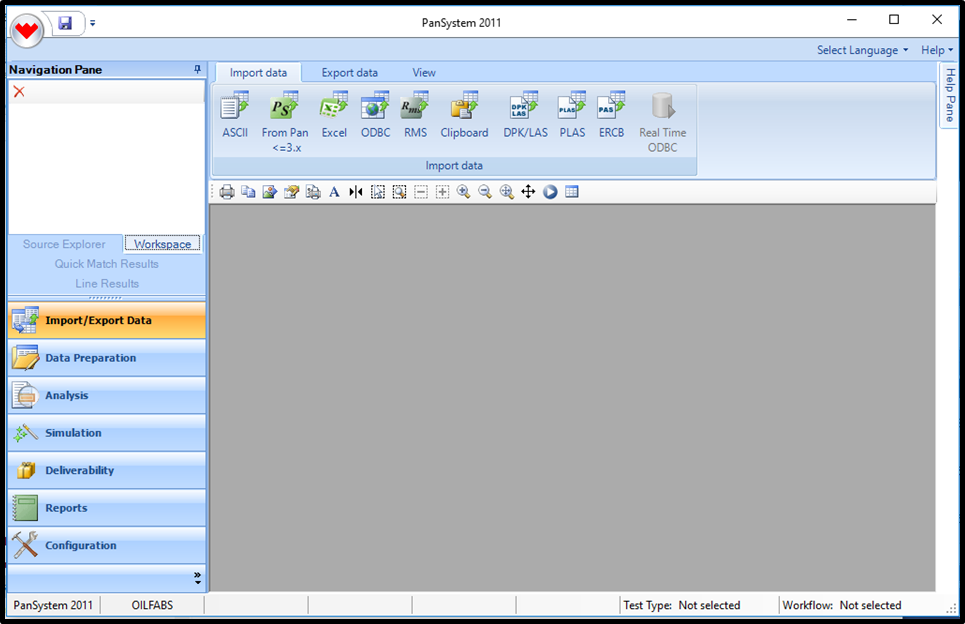
\includegraphics[scale=0.6]{welltest/interface.png}
        \caption{Giao diện phần mềm}
        \label{fig:inter_pan}
    \end{figure}
    \newpage
    \noindent
Tạo file và nhập số liệu thô như Hình \ref{fig:input_data_w} (Số liệu được tham khảo trong Applied Modern Welltest).\\
	\begin{figure}[h]
    	\centering
        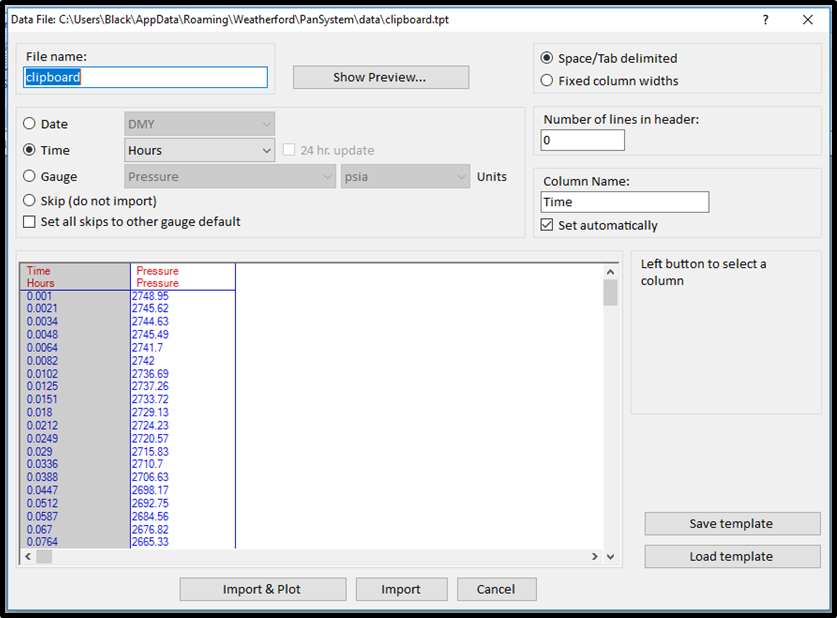
\includegraphics[scale=0.7]{welltest/input_data.png}
        \caption{Nhập số liệu}
        \label{fig:input_data_w}
    \end{figure}
    \clearpage
    \noindent
Tại thẻ \textbf{Rate Changes} nhập lại các giá trị cần thiết như Hình \ref{fig:rate_well} để chỉ rõ được \textbf{Time Period}.
	\begin{figure}[h]
    	\centering
        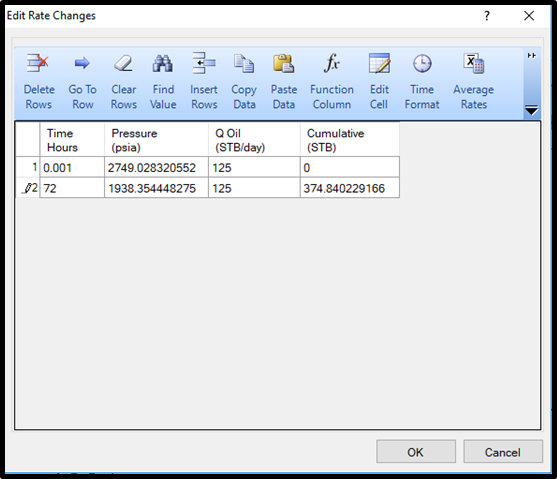
\includegraphics[scale=1]{welltest/rate_changes.png}
        \caption{Nhập Rate Changes}
        \label{fig:rate_well}
    \end{figure}
    \newpage
    \noindent
Sau khi đã thay đổi Rate changes tiếp tục nhập các thông số cần thiết khác tại thẻ \textbf{Data Preparation/ Well, reservoir \& fluid description/ Analytical Model}.
	\begin{figure}[h]
    	\centering
        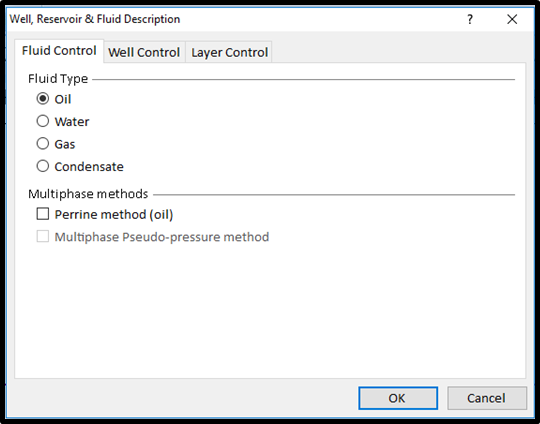
\includegraphics[scale=1]{welltest/fluid_des.png}
        \caption{Lựa chọn lưu chất phân tích}
        \label{fig:fluid_des}
    \end{figure}
    \clearpage
    \noindent
Đi đến thẻ \textbf{Well control/ Well parameters} nhập thông số bán kính giếng, Hình \ref{fig:w_radius}.
    \begin{figure}[h]
    	\centering
        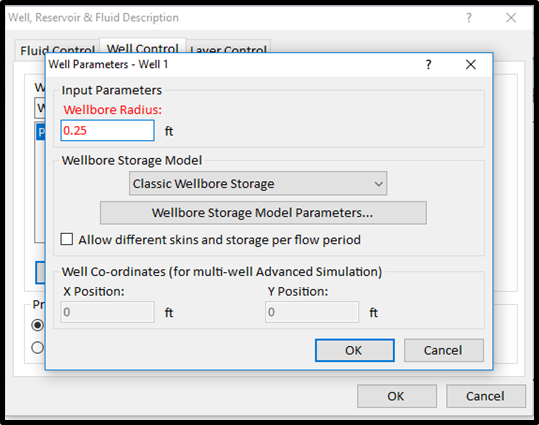
\includegraphics[scale=1]{welltest/well_radius.png}
        \caption{Nhập thông số bán kính giếng}
        \label{fig:w_radius}
    \end{figure}
    \clearpage
    \noindent
Tại thẻ \textbf{Layer control/ Layer parameters} nhập các thông số vỉa (Độ dày và độ rỗng) như Hình \ref{fig:w_layer}.
    \begin{figure}[h]
    	\centering
        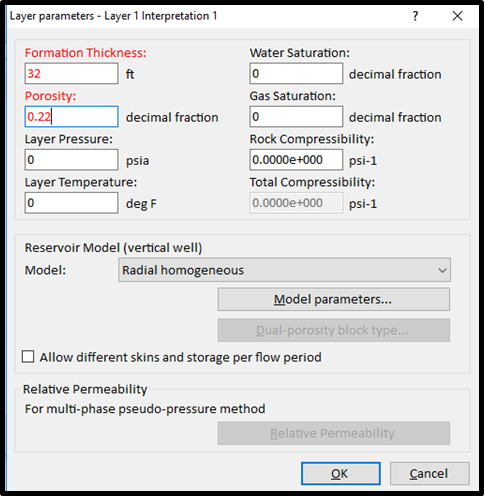
\includegraphics[scale=1]{welltest/layer_params.png}
        \caption{Các thông số vỉa}
        \label{fig:w_layer}
    \end{figure}
    \clearpage
    \noindent
Tại thẻ \textbf{Layer control/ Layer Fluid parameters} nhập các thông số hệ số thể tích thành hệ, độ nhớt của dầu và hệ số nén tổng, Hình \ref{fig:oil_params}.
    \begin{figure}[h]
    	\centering
        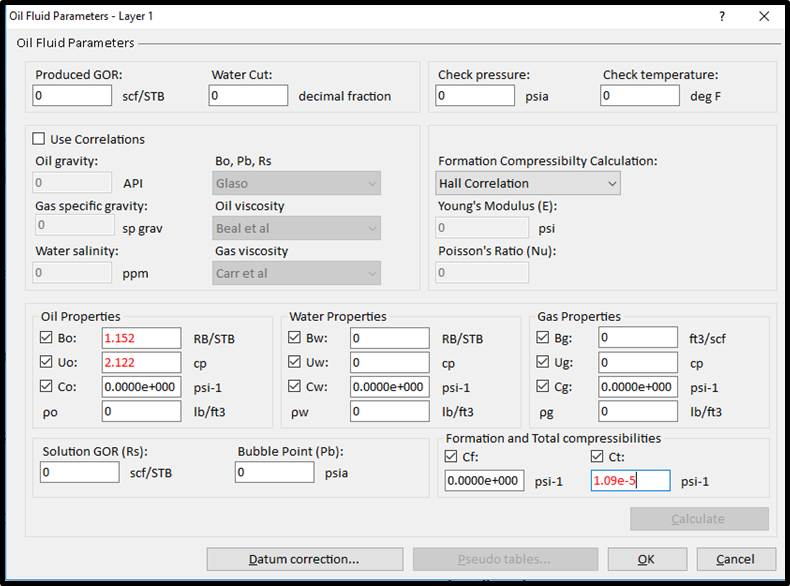
\includegraphics[scale=.7]{welltest/oil_params.png}
        \caption{Các thông số dầu}
        \label{fig:oil_params}
    \end{figure}
    \clearpage
    \noindent
Sau khi nhập đầy đủ các thông số cần thiết, quay lại thẻ \textbf{Analysis} để có thể thực hiện phân tích tính toán các thông số độ thấm, hệ số skin.\\
Trước hết thực hiện phân tích với dạng đồ thị Semi-log. Đi đến thẻ \textbf{Plot types} lựa chọn dạng đồ thị Semi-log, chọn các điểm có xu hướng nằm trên một đường thẳng và chọn công cụ \textbf{Best fit line} như Hình \ref{fig:semi_log_w}.
	\begin{figure}[h]
    	\centering
        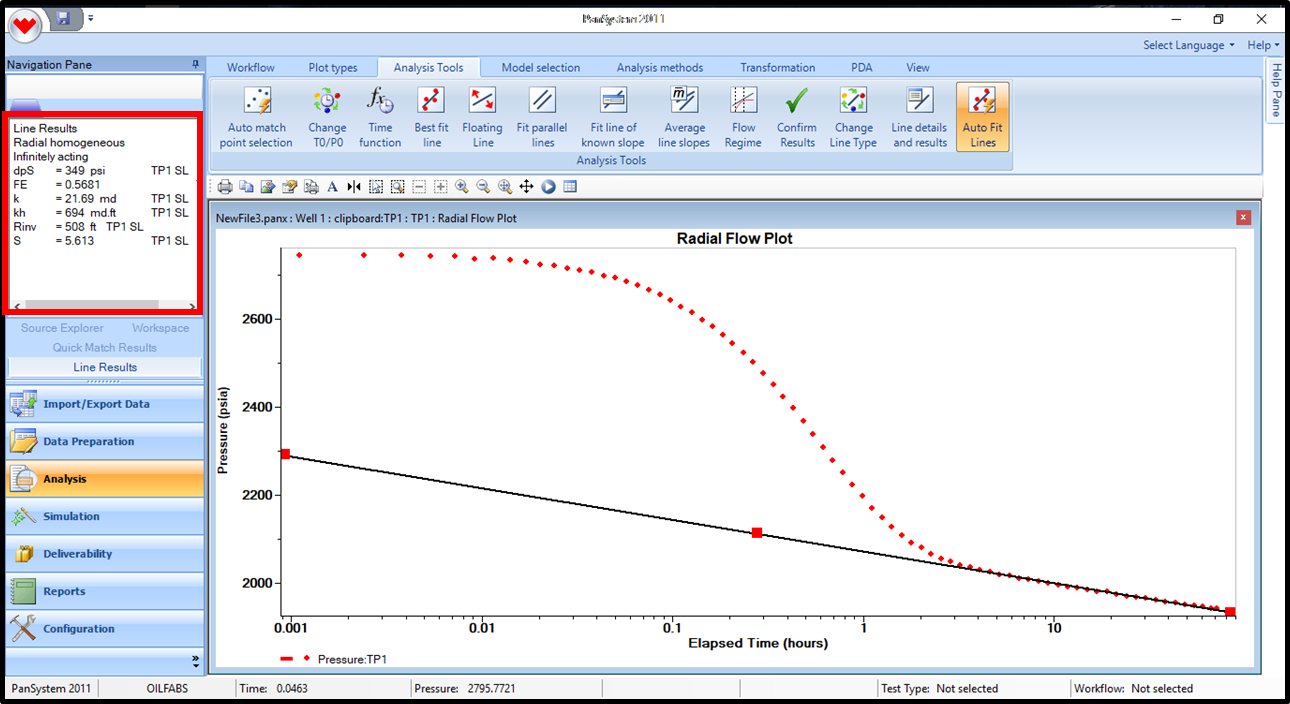
\includegraphics[scale=.45]{welltest/semilog_result.png}
        \caption{Đồ thị Semi-log và kết quả tính toán}
        \label{fig:semi_log_w}
    \end{figure}
    \newline
Các kết quả cũng được thể hiện trong Hình \ref{fig:semi_log_w} (Phần được khoanh màu đỏ) với độ thấm k = 21.69 mD, hệ số skin S = 5.61 và bán kính ảnh hưởng vào khoảng 508 ft.\\
Tiếp tục thực hiện với đồ thị Log-log nhận thêm được giá trị hệ số Wellbore storage C = 0.0053 psi/bbl. 
	\begin{figure}[h]
    	\centering
        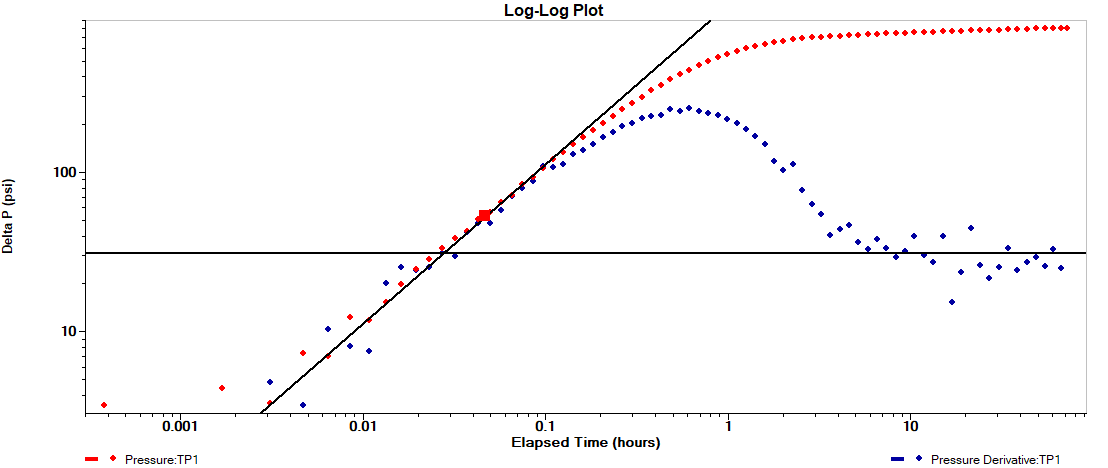
\includegraphics[scale=.4]{welltest/loglog.png}
        \caption{Đồ thị Log-log}
        \label{fig:loglog}
    \end{figure}
\section{Phương trình cân bằng vật chất}
\subsection{Tổng quan}
Phương trình cân bằng vật chất (Material Balanced Equation, MBE) được xem như là một công cụ cơ bản cho các kỹ sư công nghệ mỏ trong quá trình thực hiện phân tích và mô phỏng các tính chất vỉa.\\
Phương trình cân bằng vật chất được áp dụng để:
	\begin{itemize}
    	\item[-] Tính toán sơ bộ các thông số vỉa như lượng hydrocarbon ban đầu, kích thước mũ khí
        \item[-] Xác định sự xuất hiện, kích thước của tầng nước đáy
        \item[-] Dự đoán độ sâu của các điểm tiếp xúc giữa Gas/Oil, Oil/Water và Gas/Water
        \item[-] Dự đoán áp suất vỉa trong quá trình khai thác hay quá trình bơm ép
        \item[-] Dự đoán các đặc tính vỉa và giếng khai thác
        \item[-] Đưa ra các dữ liệu đầu vào cho quá trình mô phỏng vỉa.
    \end{itemize}
    Định nghĩa của phương trình cân bằng vật chất được giới thiệu năm 1941 bởi Schilthuis, toàn bộ vỉa được giả sử như là một bình chứa đồng nhất với áp suất trung bình vỉa P và độ bão hòa chung cho toàn vỉa, thể tích của bình chứa này luôn được bảo toàn:\\
    \hspace*{1.5cm}Thể tích ban đầu = Thể tích còn lại + Thể tích khai thác được\\
    \begin{figure}[h]
    	\centering
        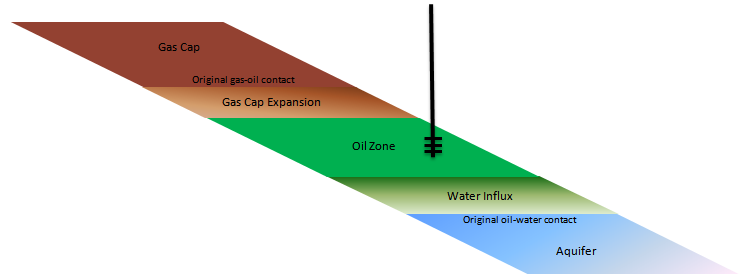
\includegraphics[scale=.7]{Fig/tank_reservoir.PNG}
        \caption{Vỉa giả sử}
    \end{figure}
	\begin{figure}[h]
    	\centering
        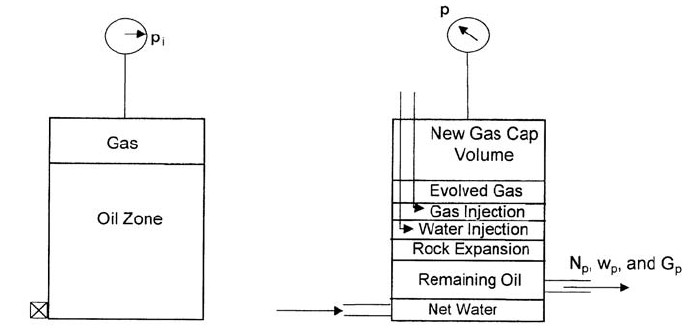
\includegraphics[scale=0.7]{Fig/tank_model.jpg}
        \caption{Mô hình cân bằng vật chất}
    \end{figure}
    \newline
    Phương trình cân bằng vật chất có thể được viết dưới dạng tổng quá như sau:\\
    \textbf{Thể tích không gian rỗng bị chiếm chỗ bởi thể tích dầu ban đầu tại áp suất $p_i$ + Thể tích không gian rỗng bị chiếm chỗ bởi khí trong mũ khí tại áp suất $p_i$ =\\
    \hspace*{1cm}Thể tích không gian rỗng bị chiếm chỗ bởi lượng dầu còn lại trong vỉa tại áp suất p\\\hspace*{1cm} + \\
    \hspace*{1cm}Thể tích không gian rỗng bị chiếm chỗ bởi khí trong mũ khí tại áp suất p\\\hspace*{1cm} + \\
    \hspace*{1cm}Thể tích không gian rỗng bị chiếm chỗ bởi sự giãn nở của khí hòa tan tại áp suất p\\\hspace*{1cm} +\\
    \hspace*{1cm}Thể tích không gian rỗng bị chiếm chỗ bởi nước xâm nhập tại áp suất p\\\hspace*{1cm} + \\
    \hspace*{1cm}Thể tích không gian rỗng thay đổi do sự giãn nở của nước liên kết và thể tích không gian rỗng giảm do sự giãn nở của đá\\\hspace*{1cm} + \\
    \hspace*{1cm}Thể tích không gian rỗng bị chiếm chỗ bởi khí bơm ép tại áp suất p\\\hspace*{1cm} +\\
    \hspace*{1cm}Thể tích không gian rỗng bị chiếm chỗ bởi nước bơm ép tại áp suất p.\\}
    Phương trình có thể được viết lại dưới dạng đơn giản như sau:
    \begin{equation}
    	F = N\times{E}_t+W_e
    \end{equation}
    Với: F = Lượng dầu khai thác được\\
    \hspace*{1cm}N = Lượng dầu ban đầu trong vỉa\\
    \hspace*{1cm}$E_t$ = Độ giãn nở tổng của chất lưu vỉa\\
    \hspace*{1cm}$W_e$ = Lượng nước xâm nhập từ tầng nước đáy\\
Phương trình cân bằng vật chất là một công cụ tuyệt vời trong quá trình "history matching" tuy nhiên không đem lại hiệu quả cao trong dự đoán đặc tính vỉa trong tương lai.
\subsection{Dự đoán đặc tính vỉa bằng MBAL}
	\subsubsection{Petroleum Experts và mô đun MBAL}
    MBAL là một mô đun được phát triển bởi Petroleum Experts, được sử dụng để phân tích cân bằng vật chất. Nguyên lý hoạt động chủ yếu dựa trên phương trình cân bằng vật chất có dạng tổng quát như sau:
    %\begin{equation}
    \begin{multline*}
    	N_p[B_o+B_g(R_p-R_s)]+W_pB_w-W_{inj}B_{winj}-G_{inj}B_{ginj}-W_eB_w\\
        = N\left\{[B_o-B_{oi}+B_g(R_{si-R_s})]+\dfrac{B_{oi}}{B_{gi}}m(B_g-B_{gi})+B_{oi}(1+m)\left(\dfrac{c_f+c_wS_w}{1-S_w}\Delta 	P\right)\right\}
	\end{multline*}
    %\end{equation}
    Một số ứng dụng của MBAL:
    \begin{itemize}
    	\item[-] Khớp lịch sử (History Matching) đặc tính vỉa để xác định lượng hydrocarbon ban đầu trong vỉa và cơ chế khai thác bằng tầng nước đáy (Aquifer)
        \item[-] Xây dựng mô hình đa vỉa (Multi-tank reservoir)
        \item[-] Phân tích đường cong suy giảm
        \item[-] Điều chỉnh các thông số PVT tương ứng với các thông số thực tế, giảm thiểu sai số trong quá trình xây dựng mô hình.
    \end{itemize}
    \newpage
	\subsubsection{Thực hành với MBAL}
Mô đun MBAL có giao diện như Hình \ref{fig:interface}.
    	\begin{figure}[h]
        	\centering
            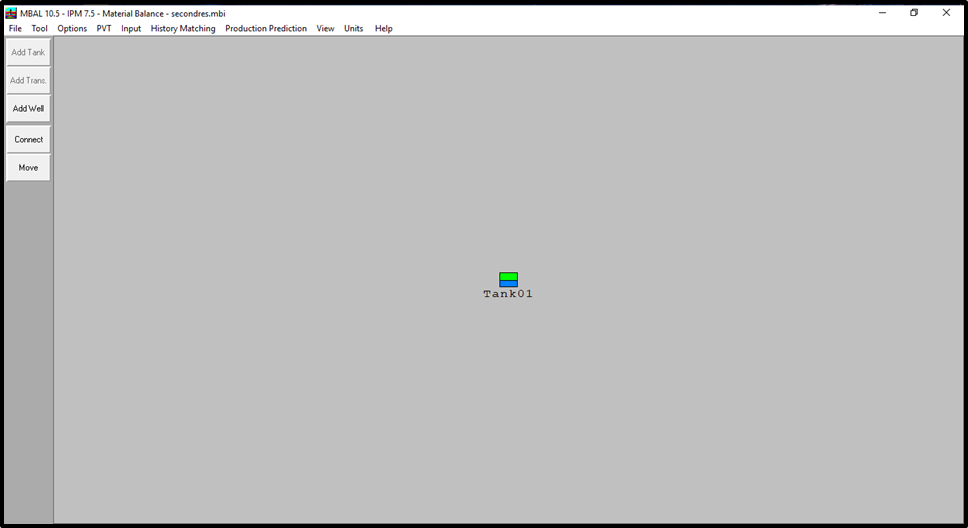
\includegraphics[scale=.6]{Fig/interface.png}
            \caption{Giao diện MBAL}
            \label{fig:interface}
        \end{figure}
        \clearpage
        \noindent
Từ giao diện, lựa chọn công cụ phân tích cân bằng vật chất tại thẻ \textbf{Tool}, Hình \ref{fig:mba_tool}.\\
		\begin{figure}[h]
        	\centering
            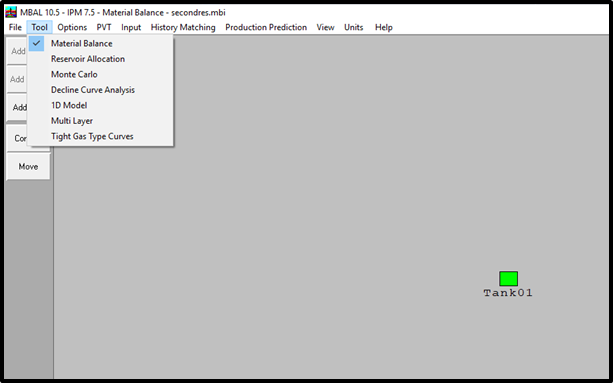
\includegraphics[scale=0.9]{Fig/mba_tool.png}
            \caption{Công cụ phân tích MBA}
            \label{fig:mba_tool}
        \end{figure}
        \clearpage
        \noindent
Nhập các thông số cần thiết (được tính toán từ thí nghiệm PVT) Hình \ref{fig:pvt_input}.
		\begin{figure}[h]
        	\centering
            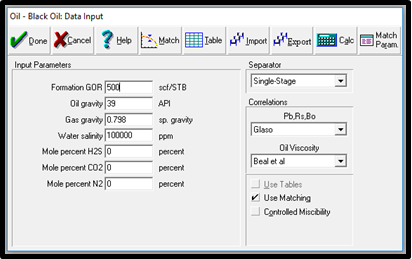
\includegraphics[scale=1.3]{Fig/pvt_input.png}
            \caption{Các thông số từ thí nghiệm PVT}
            \label{fig:pvt_input}
        \end{figure}
        \newline
Các tính dầu được xác định dựa trên mô hình Black oil. Ngoài ra, độ khoáng hóa của nước được tính toán dựa trên các tính chất của nước, khí khai thác được không chưa các thành phần $H_2S$, $CO_2$ và $N_2$.\\
Các phương trình cơ bản của mô hình Black oil:
		\begin{equation}
        	\dfrac{\partial}{\partial t}\left[\phi\left(\dfrac{S_o}{B_o}+\dfrac{R_VS_g}{B_g}\right)\right]+\nabla\left(\dfrac{1}{B_o}\vec{u}_o+\dfrac{R_V}{B_g}\vec{u}_g\right)=0
        \end{equation}
        \begin{equation}
        	\dfrac{\partial}{\partial t}\left[\phi\left(\dfrac{S_w}{B_w}\right)\right]+\nabla\left(\dfrac{1}{B_w}\vec{u}_w\right)=0
        \end{equation}
        \begin{equation}
        	\dfrac{\partial}{\partial t}\left[\phi\left(\dfrac{R_SS_o}{B_o}+\dfrac{S_g}{B_g}\right)\right]+\nabla\left(\dfrac{R_S}{B_o}\vec{u}_o+\dfrac{1}{B_g}\vec{u}_g\right)=0
        \end{equation}
\newpage
\noindent
Lựa chọn mô hình tính toán các thông số áp suất điểm bọt khí, tỉ số GOR, hệ số thành hệ, độ nhớt. Việc lựa chọn các mô hình tính toán phụ thuộc vào ba giá trị: Parameter 1, parameter 2, standard deviation được thể hiện như trong Hình \ref{fig:correlations}.
		\begin{figure}[h]
        	\centering
            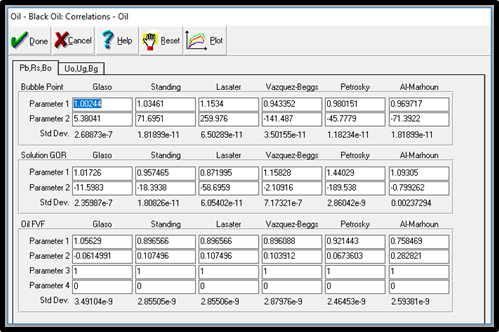
\includegraphics[scale=1.1]{Fig/correlations.png}
            \caption{Lựa chọn tương quan tính toán}
            \label{fig:correlations}
        \end{figure}
        \newline
Trong đó, giá trị Parameter 1 càng gần 0 càng tốt, giá trị Parameter 2 càng gần 1 càng tốt và giá trị Standard Deviation càng nhỏ càng tốt. Mô hình nào nhận được 2 trong 3 giá trị tốt hơn các mô hình khác sẽ được sử dụng để tính toán các áp suất điểm bọt khí, độ nhớt, tỉ số GOR và hệ số thành hệ. Đối với dữ liệu của bài toán này, mô hình Glaso sẽ được sử dụng cho việc tính toán áp suất điểm bọt khí, hệ só thể tích thành hệ, tỉ số khí-dầu; mô hình Beggs được lựa chọn để tính toán độ nhớt.
		\newpage
        \noindent
Sau khi lựa chọn được các mô hình tính toán phù hợp, thực hiện nhập các giá trị ban đầu cho mô hình vỉa, Hình \ref{fig:tank_params}. Giá trị OOIP ở đây chỉ là dự đoán sơ lược từ các dữ liệu địa chất khác.
		\begin{figure}[h]
        	\centering
            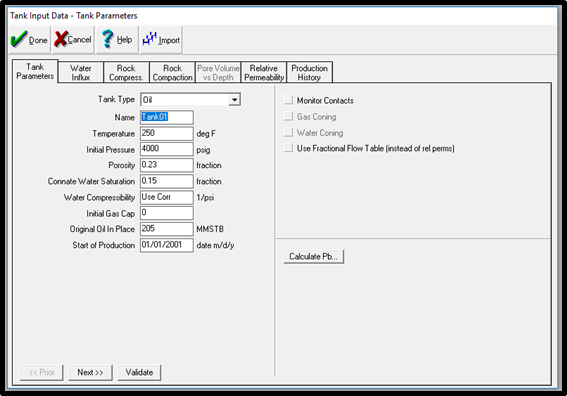
\includegraphics[scale=1]{Fig/tank_params.png}
            \caption{Các thông số ban đầu}
            \label{fig:tank_params}
        \end{figure}
        \clearpage
        \noindent
Do không có thông số nào chứng tỏ vỉa có sự tồn tại của tầng nước đáy nên thẻ \textbf{Water Influx} được bỏ trống.
		\begin{figure}[h]
        	\centering
            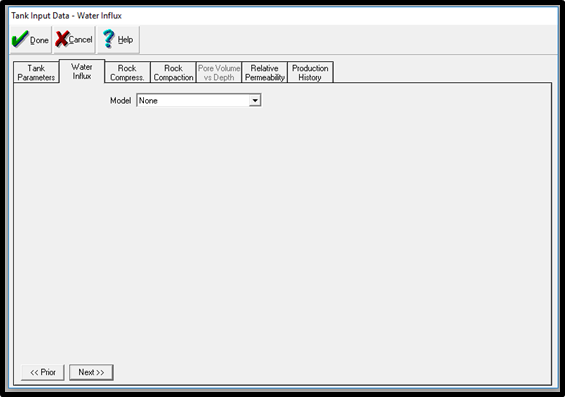
\includegraphics[scale=1]{Fig/water_influx.png}
            \caption{Water Influx}
            \label{fig:water_influx}
        \end{figure}
        \clearpage
        \noindent
Độ nén của đá được tính toán dựa trên các tương quan.
		\begin{figure}[h]
        	\centering
            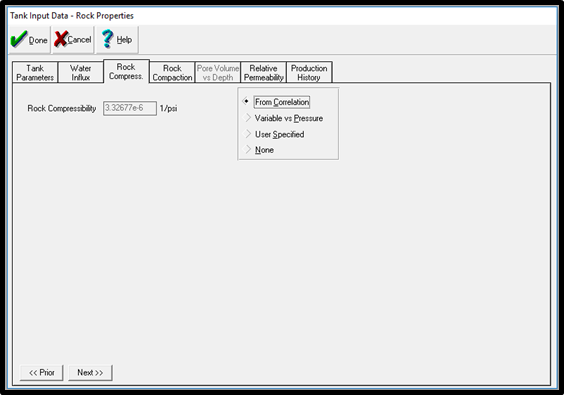
\includegraphics[scale=1]{Fig/compress.png}
            \caption{Độ nén đá}
            \label{fig:compress}
        \end{figure}
        \clearpage
        \noindent
Tiếp tục nhập các giá trị độ thấm tương đối.
		\begin{figure}[h]
        	\centering
            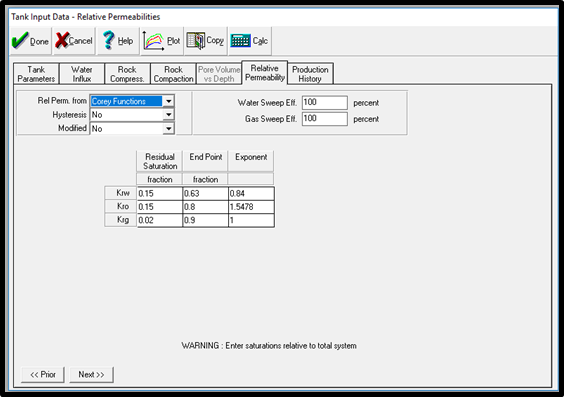
\includegraphics[scale=1]{Fig/rel_perm.png}
            \caption{Độ thấm tương đối}
            \label{fig:rel_perm}
        \end{figure}
        \clearpage
        \noindent
Dữ liệu cuối cùng cần được đưa vào là các giá trị khai thác trong lịch sử như Hình \ref{fig:pro_history}
		\begin{figure}[h]
        	\centering
            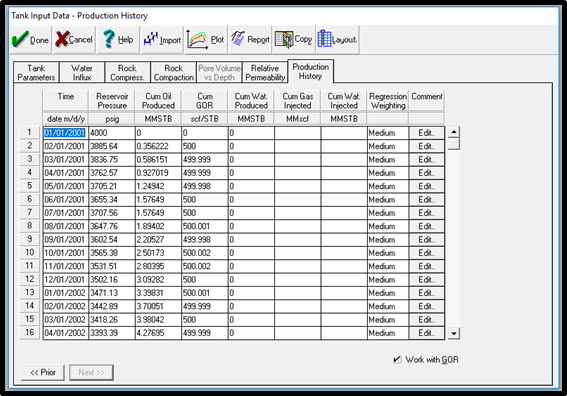
\includegraphics[scale=1]{Fig/Pro_history.png}
            \caption{Lịch sử khai thác}
            \label{fig:pro_history}
        \end{figure}
		\clearpage
        \noindent
Sau khi nhập đầy đủ các dữ liệu cần thiết, quay lại giao diên tổng để tiếp tục thực hiện khớp lịch sử. Tại thẻ \textbf{History Matching} lựa chọn \textbf{All} nhận được các đồ thị như sau:
		\begin{figure}[h]
        	\centering
            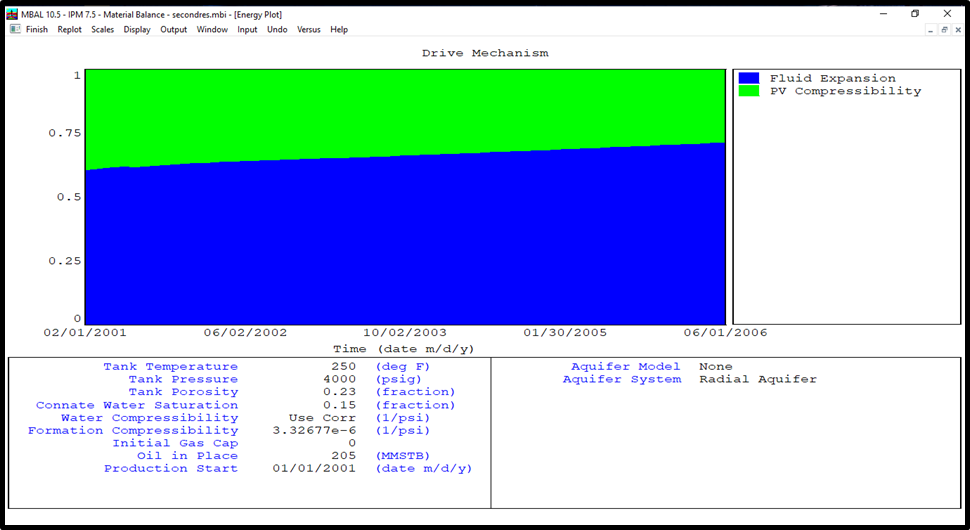
\includegraphics[scale=0.6]{Fig/drive_mechanism.png}
            \caption{Cơ chế năng lượng vỉa}
            \label{fig:drive_mech}
        \end{figure}
        \begin{figure}[h]
        	\centering
            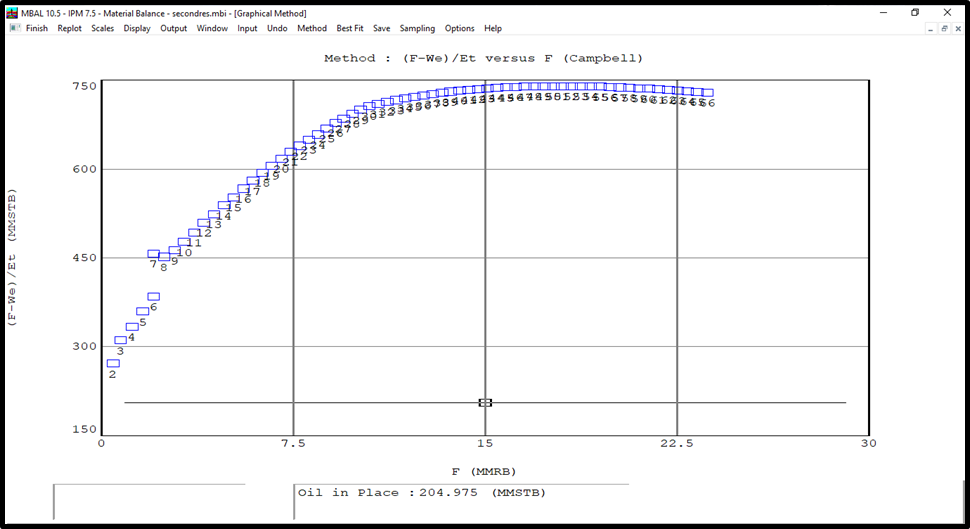
\includegraphics[scale=0.6]{Fig/gra_method.png}
            \caption{Phương pháp Graphical}
            \label{fig:gra_method}
        \end{figure}
        \begin{figure}[h]
        	\centering
            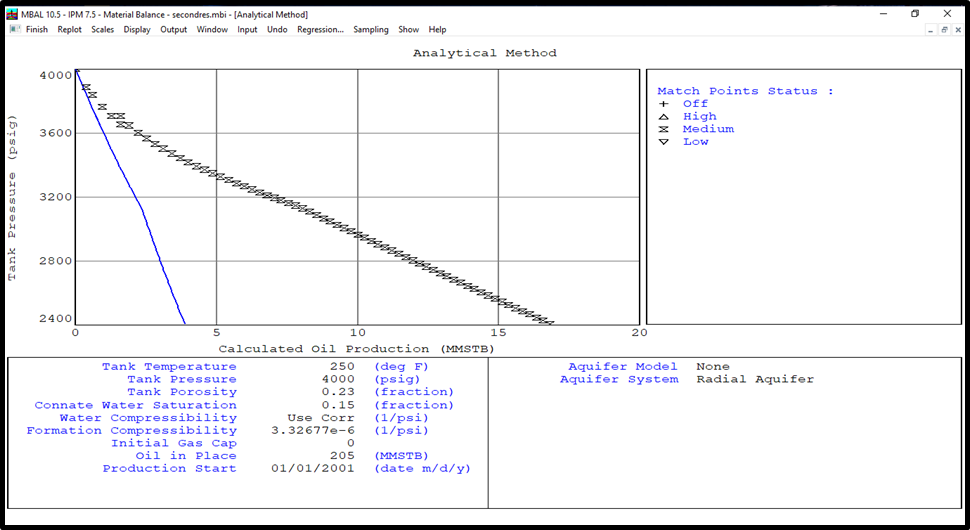
\includegraphics[scale=0.6]{Fig/analytical_method.png}
            \caption{Phương pháp Analytical}
            \label{fig:ana_method}
        \end{figure}
        \clearpage
        \noindent
Trong đó Hình \ref{fig:drive_mech} thể hiện mối quan hệ giữa các cơ chế năng lượng vỉa, Hình \ref{fig:gra_method} dự đoán cơ chế thu hồi có thế thực hiện, Hình \ref{fig:ana_method} cho thấy mức độ thay đổi của áp suất vỉa theo lượng dầu khai thác được đối với mô hình đang xét.\\
Lưu ý rằng, phương pháp Graphical Hình \ref{fig:gra_method} chính là đồ thị Campbell dự đoán các cơ chế khai thác (Hình \ref{fig:campbell_plot}). Dựa vào cả hai đồ thị này thấy được ở mô hình vỉa đang xét có sự xuất hiện của cơ chế năng lượng tầng nước đáy. 
		\begin{figure}[h]
        	\centering
            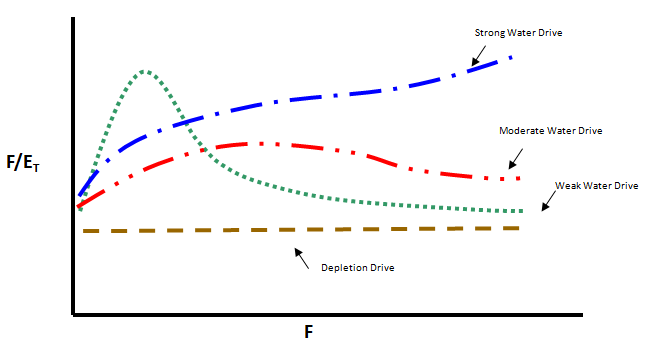
\includegraphics[scale=1]{Fig/Campbell.png}
            \caption{Đồ thị Campbell}
            \label{fig:campbell_plot}
        \end{figure}
        \newline
Tuy nhiên, đồ thị cơ chế năng lượng vỉa Hình \ref{fig:drive_mech} lại không thể hiện sự xuất hiện của tâng nước đáy, do đó \textbf{Water Influx} cần phải được lựa chọn là một thông số đầu vào của mô hình vỉa.
		\begin{figure}[h]
        	\centering
            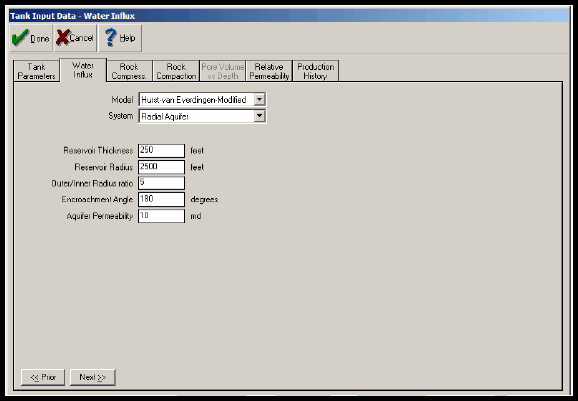
\includegraphics[scale=1]{Fig/water_influx_1.png}
            \caption{Lựa chọn mô hình Water Influx}
            \label{fig:aquifer_model}
        \end{figure}
Tương quan được lựa chọn để tính toán là Hurst-van Everdinger-Modified với các thông số như Hình \ref{fig:aquifer_model}.
		\newpage
        \noindent
Thực hiện lại quá trình khớp lịch sử cho mô hình mới thu được các đồ thị sau:
        \begin{figure}[h]
        	\centering
            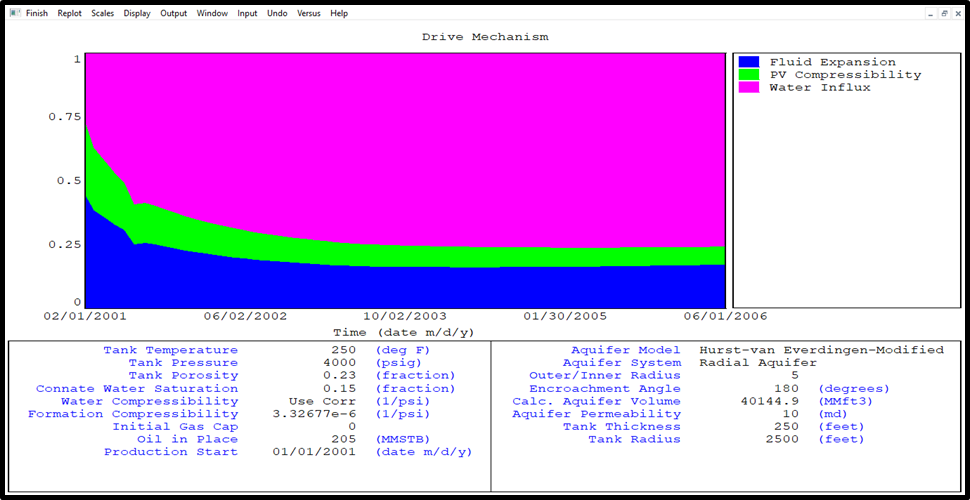
\includegraphics[scale=0.6]{Fig/ener_aquifer.png}
            \caption{Cơ chế năng lượng vỉa}
            \label{fig:ener_aquifer}
        \end{figure}
        \begin{figure}[h]
        	\centering
            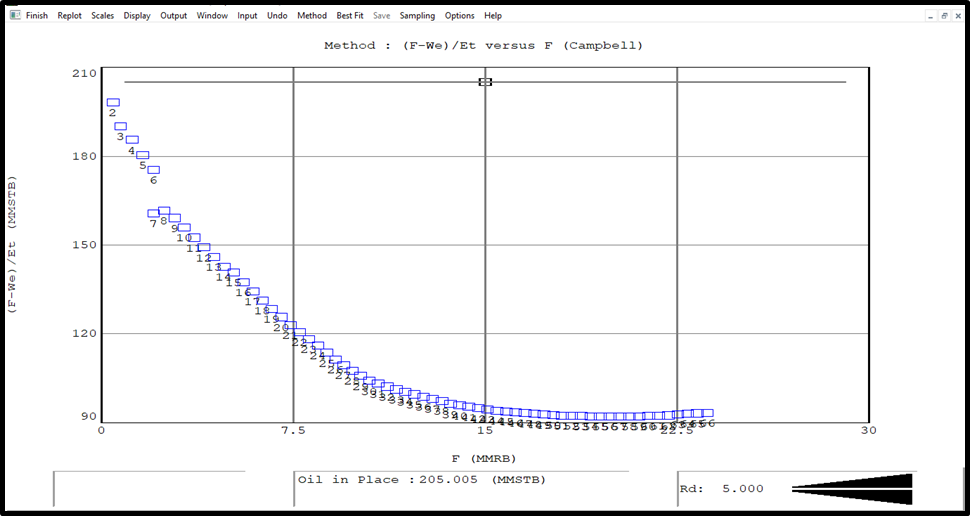
\includegraphics[scale=0.6]{Fig/gra_aquifer.png}
            \caption{Phương pháp Graphical}
            \label{fig:gra_aquifer}
        \end{figure}
        \begin{figure}[h]
        	\centering
            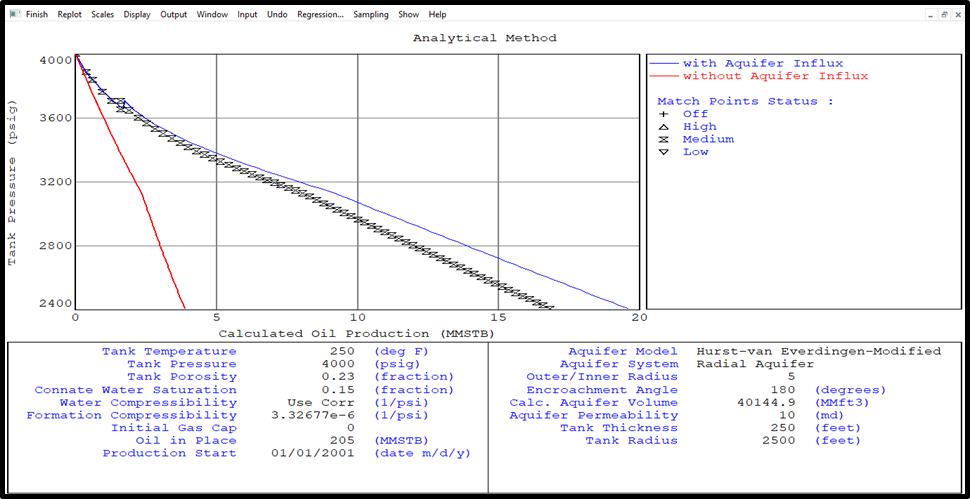
\includegraphics[scale=0.6]{Fig/ana_aquifer.png}
            \caption{Phương pháp Analytical}
            \label{fig:ana_aquifer}
        \end{figure}
        \begin{figure}[h]
        	\centering
            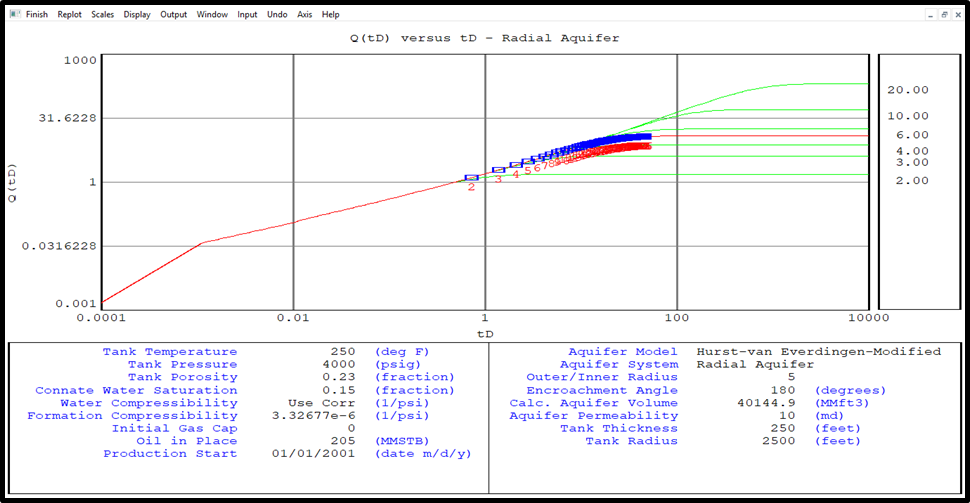
\includegraphics[scale=0.6]{Fig/wd_aquifer.png}
            \caption{Lưu lượng tầng nước đáy}
            \label{fig:wd_aquifer}
        \end{figure}
        \clearpage
        \noindent
Đồ thị Hình \ref{fig:ana_aquifer} cho thấy rằng đối với mô hình tầng nước đáy đăng xét, mô hình tính toán dự đoán lưu lượng khai thác lớn hơn so với thực tế quan sát được. Cần phải thực hiện tinh chỉnh lại dữ liệu đầu vào để mô hình đưa ra được kết quả chính xác hơn. Công việc này có thể được thực hiện tại thẻ \textbf{Regression...} ở đồ thị Analytical. Sau khi lựa chọn thẻ \textbf{Regression...} chương trình sẽ hiển thị cửa sổ như như Hình \ref{fig:before_reg}, tích vào những lựa chọn cần thiết cho tinh chỉnh dữ liêu (Oil in Place, Outer/Inner Radius, Encroachment Angle, Aquifer Permeability):
		\begin{figure}[h]
        	\centering
            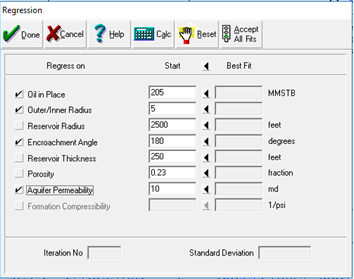
\includegraphics[scale=1.6]{Fig/before_regression.png}
            \caption{Thực hiện hồi quy tinh chỉnh dữ liệu đầu vào}
            \label{fig:before_reg}
        \end{figure}
        \clearpage
        \begin{figure}[h]
        	\centering
            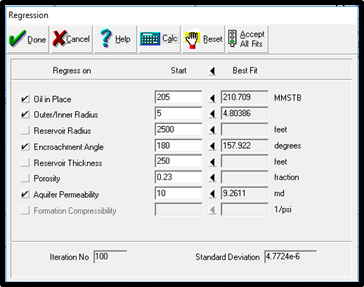
\includegraphics[scale=1.6]{Fig/after_regression.png}
            \caption{Kết quả sau hồi quy}
            \label{fig:after_reg}
        \end{figure}
        \noindent
Hình \ref{fig:after_reg} thể hiện kết quả nhận được sau khi thực hiện hồi quy tỉnh số liệu đầu vào. Tiếp tục thực hiện khớp lịch sử với những dữ liệu đầu vào mới này nhận được kết quả như sau:
		\begin{figure}[h]
        	\centering
            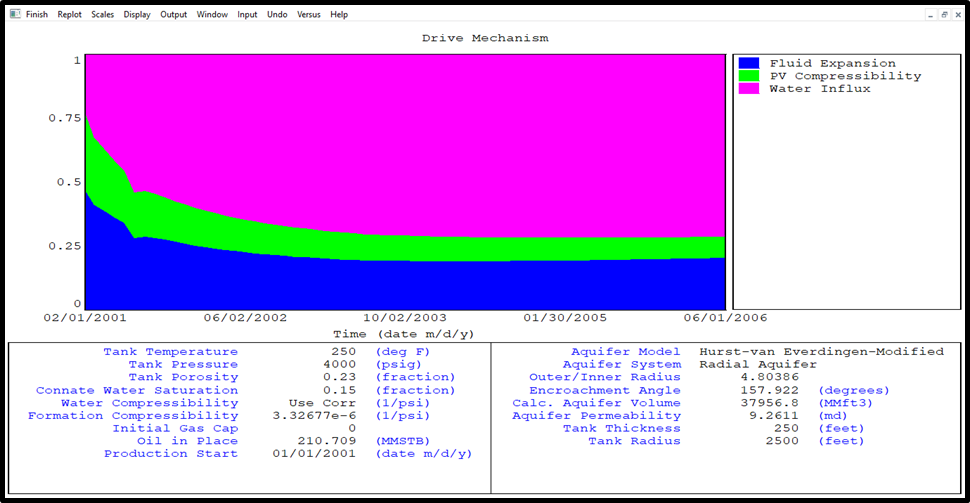
\includegraphics[scale=0.6]{Fig/ener_fixed.png}
            \caption{Cơ chế năng lượng vỉa}
            \label{fig:ener_fixed}
        \end{figure}
        \begin{figure}[h]
        	\centering
            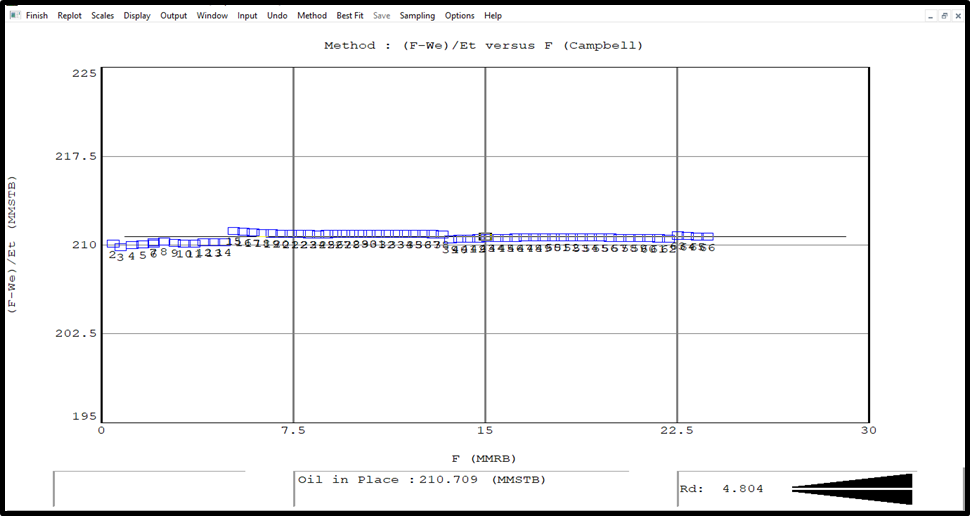
\includegraphics[scale=0.6]{Fig/gra_fixed.png}
            \caption{Phương pháp Graphical}
            \label{fig:gra_fixed}
        \end{figure}
        \begin{figure}[h]
        	\centering
            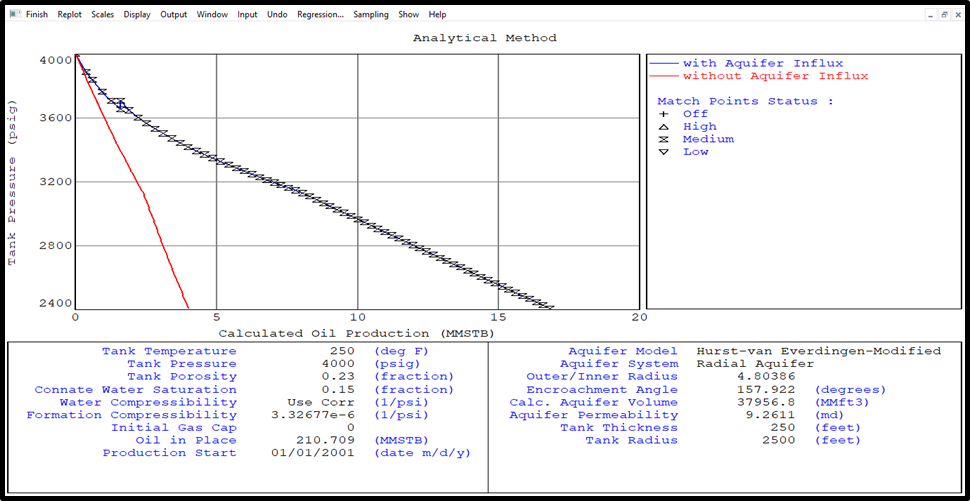
\includegraphics[scale=0.6]{Fig/ana_fixed.png}
            \caption{Phương pháp Analytical}
            \label{fig:ana_fixed}
        \end{figure}
        \begin{figure}[h]
        	\centering
            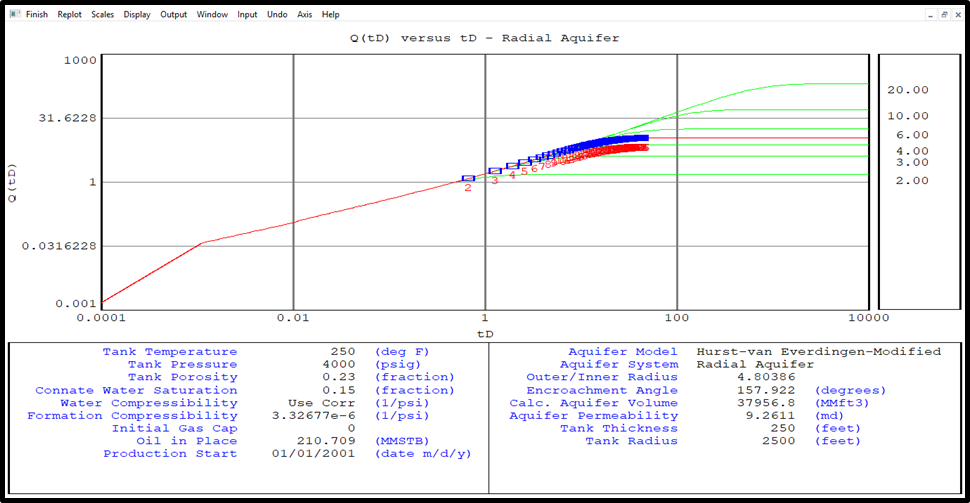
\includegraphics[scale=0.6]{Fig/wd_fixed.png}
            \caption{Lưu lượng tầng nước đáy}
            \label{fig:wd_fixed}
        \end{figure}
        \clearpage
        \noindent
Mô hình đạt được hiện tại cho thấy sự chính xác hơn về lưu lượng khai thác dự đoán với trong thực tế quan sát được. Có thể đưa ra được những kết luận như sau:
	\begin{itemize}
    	\item[-] OOIP = 210.709 (MMSTB)
        \item[-] Cơ chế năng lượng vỉa bao gồm: Sự giãn nở của lưu chất vỉa, sự nén của không gian rỗng trong vỉa, sự thâm nhập của tầng nước đáy
        \item[-] Cơ chế thu hồi dầu có thể được sử dụng là \textit{Depletion Drive}
    \end{itemize}
\section{Mô phỏng vỉa}
\subsection{Tổng quan}
Mô phỏng vỉa là quá trình xây dựng những mô hình có khả năng tính toán định lượng và minh giải những thông số vỉa (tĩnh và động) có xu hướng thay đổi trong tương lai.\\
Mô phỏng vỉa cần phải được thực hiện để có thể xác định được chiến lược lâu dài cho toàn vỉa:
	\begin{itemize}
    	\item[-] Đánh giá vỉa
        	\begin{itemize}
            	\item[+] Xác định trữ lượng có khả năng thu hồi được một cách chính xác nhất
            \end{itemize}
        \item[-] Quản lý vỉa
        	\begin{itemize}
            	\item[+] Đưa ra phương pháp mang lại hiệu quả kinh tế tốt nhất, số lượng giếng, vị trí đặt giếng và lưu lượng bơm ép
                \item[+] Đưa ra cơ sở hạ tầng phù hợp
            \end{itemize}
		\item[-] Kiểm soát những yếu tố không mong muốn
        	\begin{itemize}
            	\item[+] Đánh giá rủi ro kinh tế trong quá trình thăm dò và giai đoạn sớm của vỉa
                \item[+] Đánh giá mức độ ảnh hưởng của đối tượng không mong muốn (early gas, water breakthrough, coning).
            \end{itemize}
    \end{itemize}
Mô hình thông dụng:
	\begin{itemize}
    	\item[-] Mô hình giải tích
        \item[-] Mô hình số học
    \end{itemize}
Cả hai mô hình trên đều thuộc về phương pháp mô phỏng sử dụng mô hình toán học.\\
Mô hình giải tích thường được sử dụng cho các vỉa đơn giản, dựa trên những phương pháp phân tích có thể tính toán trực tiếp kết quả như:
	\begin{itemize}
    	\item[-] Phương trình cân bằng vật chất
        \item[-] Đường cong suy giảm
        \item[-] Mô phỏng tầng nước đáy (Aquifer)
        \item[-] Phân tích thử vỉa
    \end{itemize}
Mô hình số học được sử dụng cho những vỉa phức tạp, có những mô tả về dòng chảy lưu chất trong vỉa, thường sử dụng những phương pháp đưa ra kết quả gần đúng:
	\begin{itemize}
    	\item[-] Phương pháp sai phân hữu hạn
        \item[-] Mô hình thủy động lực quanh giếng
    \end{itemize}

Về cơ bản, quy trình mô phỏng được thực hiện theo sơ đồ Hình \ref{fig:workflow}.
	\begin{figure}[h]
    	\centering
        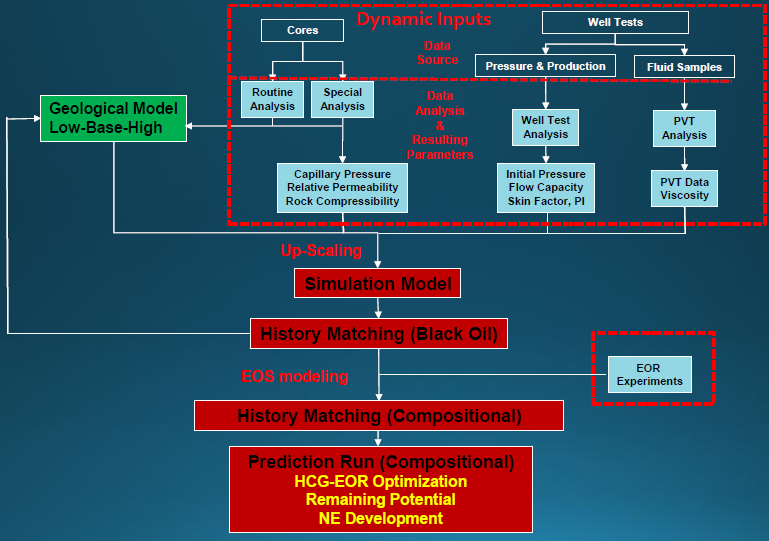
\includegraphics[scale=.7]{Fig/model_workflow.PNG}
        \caption{Quy trình mô phỏng vỉa}
        \label{fig:workflow}
    \end{figure}
\subsection{Mô phỏng vỉa với phần mềm ECLIPSE}
    \subsubsection{ECLIPSE}
Chức năng cơ bản:
	\begin{enumerate}
    	\item[-] Đánh giá các kịch bản phát triển mỏ
        \item[-] Thiết kế vị trí giếng khoan mới
        \item[-] Đánh giá kế quả khai thác
        \item[-] Đặt lại vị trí giếng khoan cũ
        \item[-] Kiểm tra lại.
    \end{enumerate}
Quá trình giải bài toán sai phân hữu hạn cũng được coi như là quá trình xử lý bài toán về các thành phần lưu chất, do đó, các mô hình mô phỏng được giới thiệu trong ECLIPSE cũng đồng thời dựa trên trên kĩ thuật tìm nghiệm cho bài toán sai phân hữu hạn.\\
Mô hình mô phỏng Black Oil:
	\begin{itemize}
    	\item[-] Hai pha dầu-khí có mặt trong vỉa được xét như là một thành phần
        \item[-] Giả sử các thành phần của dầu và khí không thay đổi theo áp suất và thời gian.
    \end{itemize}
Mô hình mô phỏng Compositional:
	\begin{itemize}
    	\item[-] Pha dầu và pha khí được xét là là hỗn hợp đa thành phần
        \item[-] Lưu chất vỉa trong mọi điều kiện nhiệt độ, áp suất, thành phần, thời gian được đặc trưng bởi phương trình trạng thái.
    \end{itemize}  
\chapter{KẾT LUẬN VÀ KIẾN NGHỊ}
\section{Kết luận}
Trong thời gian thực tập tại Công ty Dầu khí Việt-Nhật, về cơ bản em đã hoàn thành được một số nhiệm vụ đã đề ra:
	\begin{itemize}
    	\item[-] Tìm hiểu về Công ty và các hoạt động hiện tại
        \item[-] Tìm hiểu về phân tích thử vỉa, phân tích cân bằng vật chất và mô phỏng vỉa
        \item[-] Làm quen với các phần mềm, mô đun phân tích chuyên dụng như PanSystem, MBAL, ECLIPSE.
    \end{itemize}
\section{Kiến nghị}
Qua quá trình thực tập em nhận thấy kiến thức được học tại Trường còn rất giới hạn, mong rằng các Thầy, Cô bộ môn sẽ sắp xếp để có thể truyền đạt thêm nhiều kiến thức hơn nữa cho sinh viên trong quãng thời gian sắp tới.
\end{document}
